\section{Pile-up tracks rejection using timing informations}
\label{sec:purej}
An essential step in rejecting pileup is to exclude from relevant
quantities charged particles which are not associated with the hard
interaction.  
This step is critical to maintain the performance of charged isolation
sums for leptons, b-tagging, and the charged component of jets and
missing transverse momentum.  
One method commonly used in CMS  to associate tracks with the hard
primary vertex, PV, is a simple selection on the distance between the
track and the vertex, $|\Delta
z(\textnormal{track},\textnormal{PV})|<1$~mm, which maintains 
high efficiency for charged particles actually originating from the
hard interaction. 
To optimize this seleciton, the isolation sum of charged
particles was studied in 200 pileup collisions for $|\Delta z|$
ranging between 0.2 and 2~mm. 
For particles at any pseudorapidity within the barrel acceptance, a
selection window of 1~mm maximizes the identification performance
(measured by the ROC curve).  
In the endcaps, a slightly looser selection may provide a better
performance, with 1~mm being close to optimal. 
Hence, for an interaction density in excess of 1.0~event/mm,
corresponding to operations at approximately 100 pileup and above,
some or many of the resulting tracks will be associated with the 
hard primary vertex, contaminating the set of tracks used to calculate
the relevant physics quantities and degrading the performance.

This effect is most directly quantified as a function of the line
density of events along the beam line, which drives the probability
that additional vertices will be close enough in space to the hard
interaction to contaminate the set of associated tracks with those
from pileup. 
This association method can be extended with precision timing, by
adding a requirement on the time distance $|\Delta
t(\textnormal{track},\textnormal{PV})|<N\times\sigma_t^{\textnormal{track}}$ for those tracks with valid timing information.  Tracks without valid timing information are retained.
In this study,  $N = 3$ is used together with an average time resolution $\sigma_t=35$~ps for tracks with valid timing information, corresponding to the requirement 
$|\Delta t(\textnormal{track},\textnormal{PV})|<105$~ps.

Using this association criterion, the efficiency for reconstructing and
associating tracks from pileup interactions in \ttbar events is
shown in Fig.~\ref{fig:trkvtx}, both with and without precision
timing, as a function of the event line density. The effect of timing
on signal tracks for these processes  has been studied as well, and in
zero-pileup conditions shows no significant impact on the association
efficiency. 

The left panel of the figure shows the results obtained with the full
simulation and reconstruction described in this TDR, while the right
panel shows results from the fast-simulation, where the time smearing
is applied at the vertex. A fair agreement is observed in the
reduction of wrong associations for comparable assumption on the
timing resolution and efficiency. This provides confidence in the use of the fast
simulation adopted for some of the performance analyses presented in
the TDR.  

\begin{figure}[hbtp]
\centering
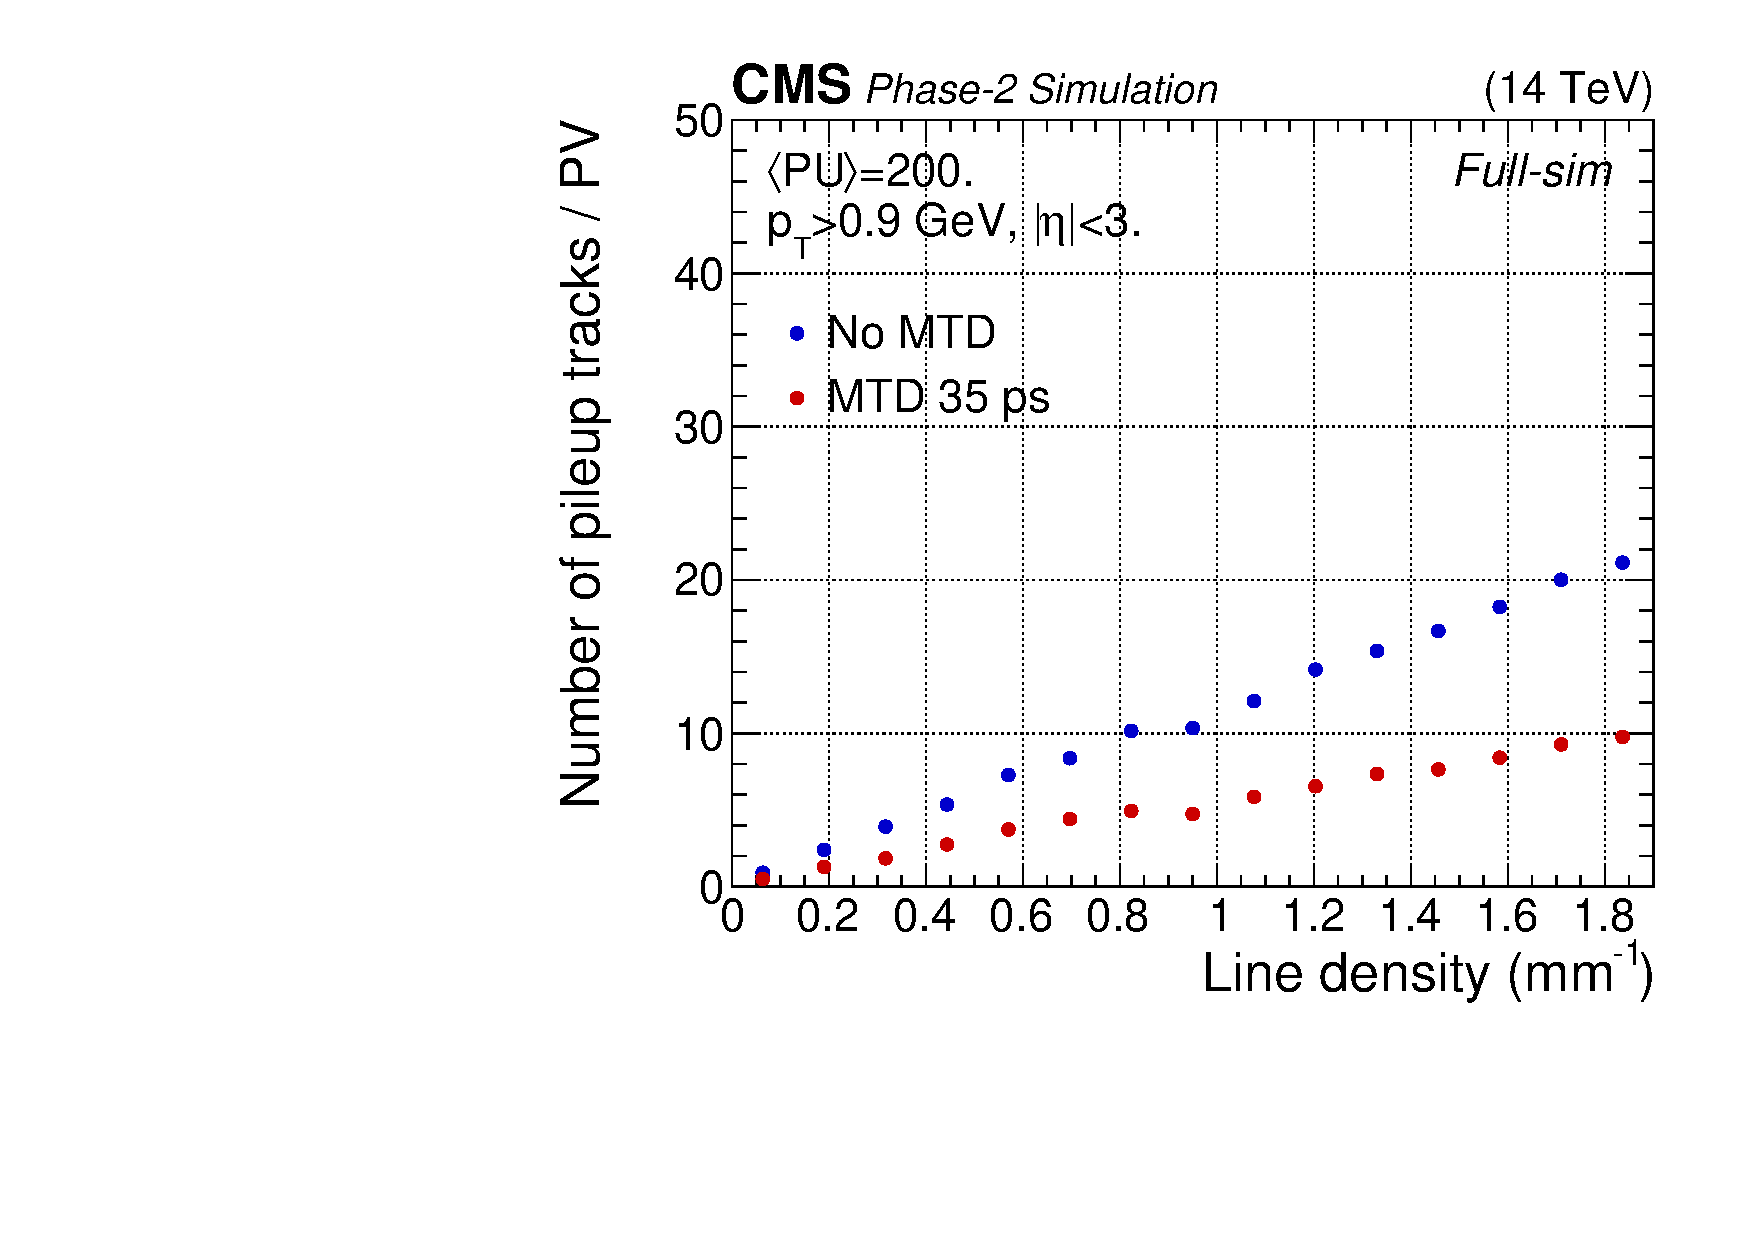
\includegraphics[width=0.48\textwidth]{fig/performance/purej/ForApproval/track_pu_vs_linden_nugun_nobdt.pdf}
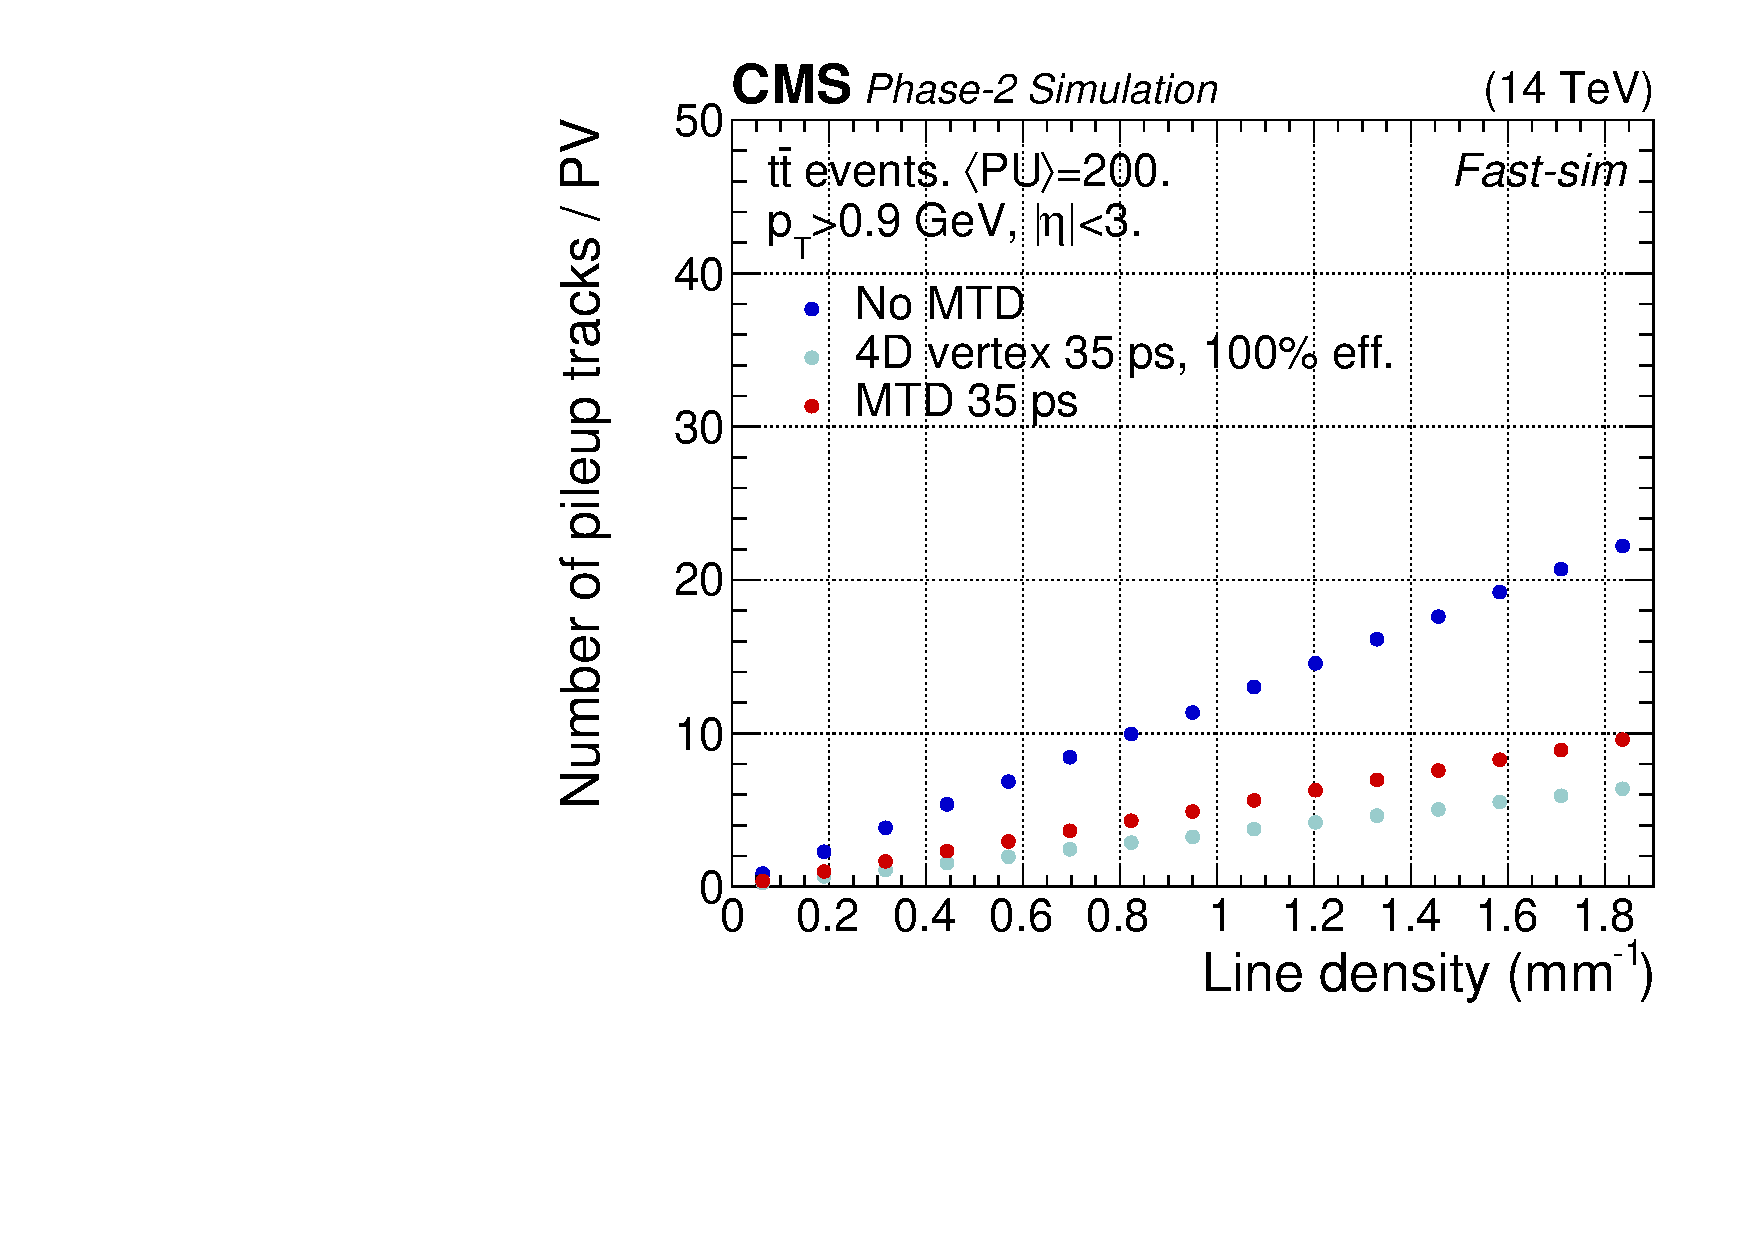
\includegraphics[width=0.48\textwidth]{fig/performance/purej/ForApproval/nputracks_fastsim.pdf}
 \caption{Left: Number of tracks from pileup incorrectly 
   associated with the hard primary vertex in \ttbar events from full
   simulation as a function of the pileup density, shown with (4D vtx)
   and without (3D vtx) precision timing. Right: Ditto for
   fast-simulation and different assumption on the time association efficiency.}
   \label{fig:trkvtx}
\end{figure}

With fast-sim is possible to estimate the effect of the reduction of the track-MTD association efficiency, which is about 30\% for the efficiency which is currently achieved in the MTD full simulation and reconstruction. As we have discussed, there are margins to to improve the tracking algorithm and MTD association at PU200, with direct benefits to this figure of merit. 

Fig.\ref{fig:purej_bdt} (left) reports also the rejection which can be achieved using a multivariate classifier for the tracks. The multivariate classifier is trained on tracks from TTbar events at PU200, separating them in 2 species, primary vertex tracks and PU tracks. A boosted decision tree is trained using as inputs track quality input parameters (number of track hits, $\chi^2$, $p_{T}$, $\eta$), track-MTD matching variables ($\chi^2_{space}$,$\chi^2_{time}$), and the $\delta_{t}$ at vertex. The impact parameters of the track with respect to the vertex are not fed to the BDT to allow only selection on the timing information. The purpose of this classifier is to reject the residual fake-MTD track associations discussed in section~\ref{C5Sec:mtdreco} at PU200 when applying only a beam spot constraint, in order to reduce the over-cleaning for tracks belonging to the primary vertex. The effectiveness of this approach is shown in Fig.~\ref{fig:purej_bdt}, which compares the efficiency for tracks matched to a primary vertex generator particle, as a function of $\pt$ and $\eta$. The efficiency loss from the straight $\delta_{t}<3\sigma_{t}$ cut is reduced by the BDT approach, which has a small efficiency loss compared to the $d_{z}$ cut, and a rejection comparable to the $\delta_{z}+\delta_{t}$ cut. 

\begin{figure}[!phtb]
\centering
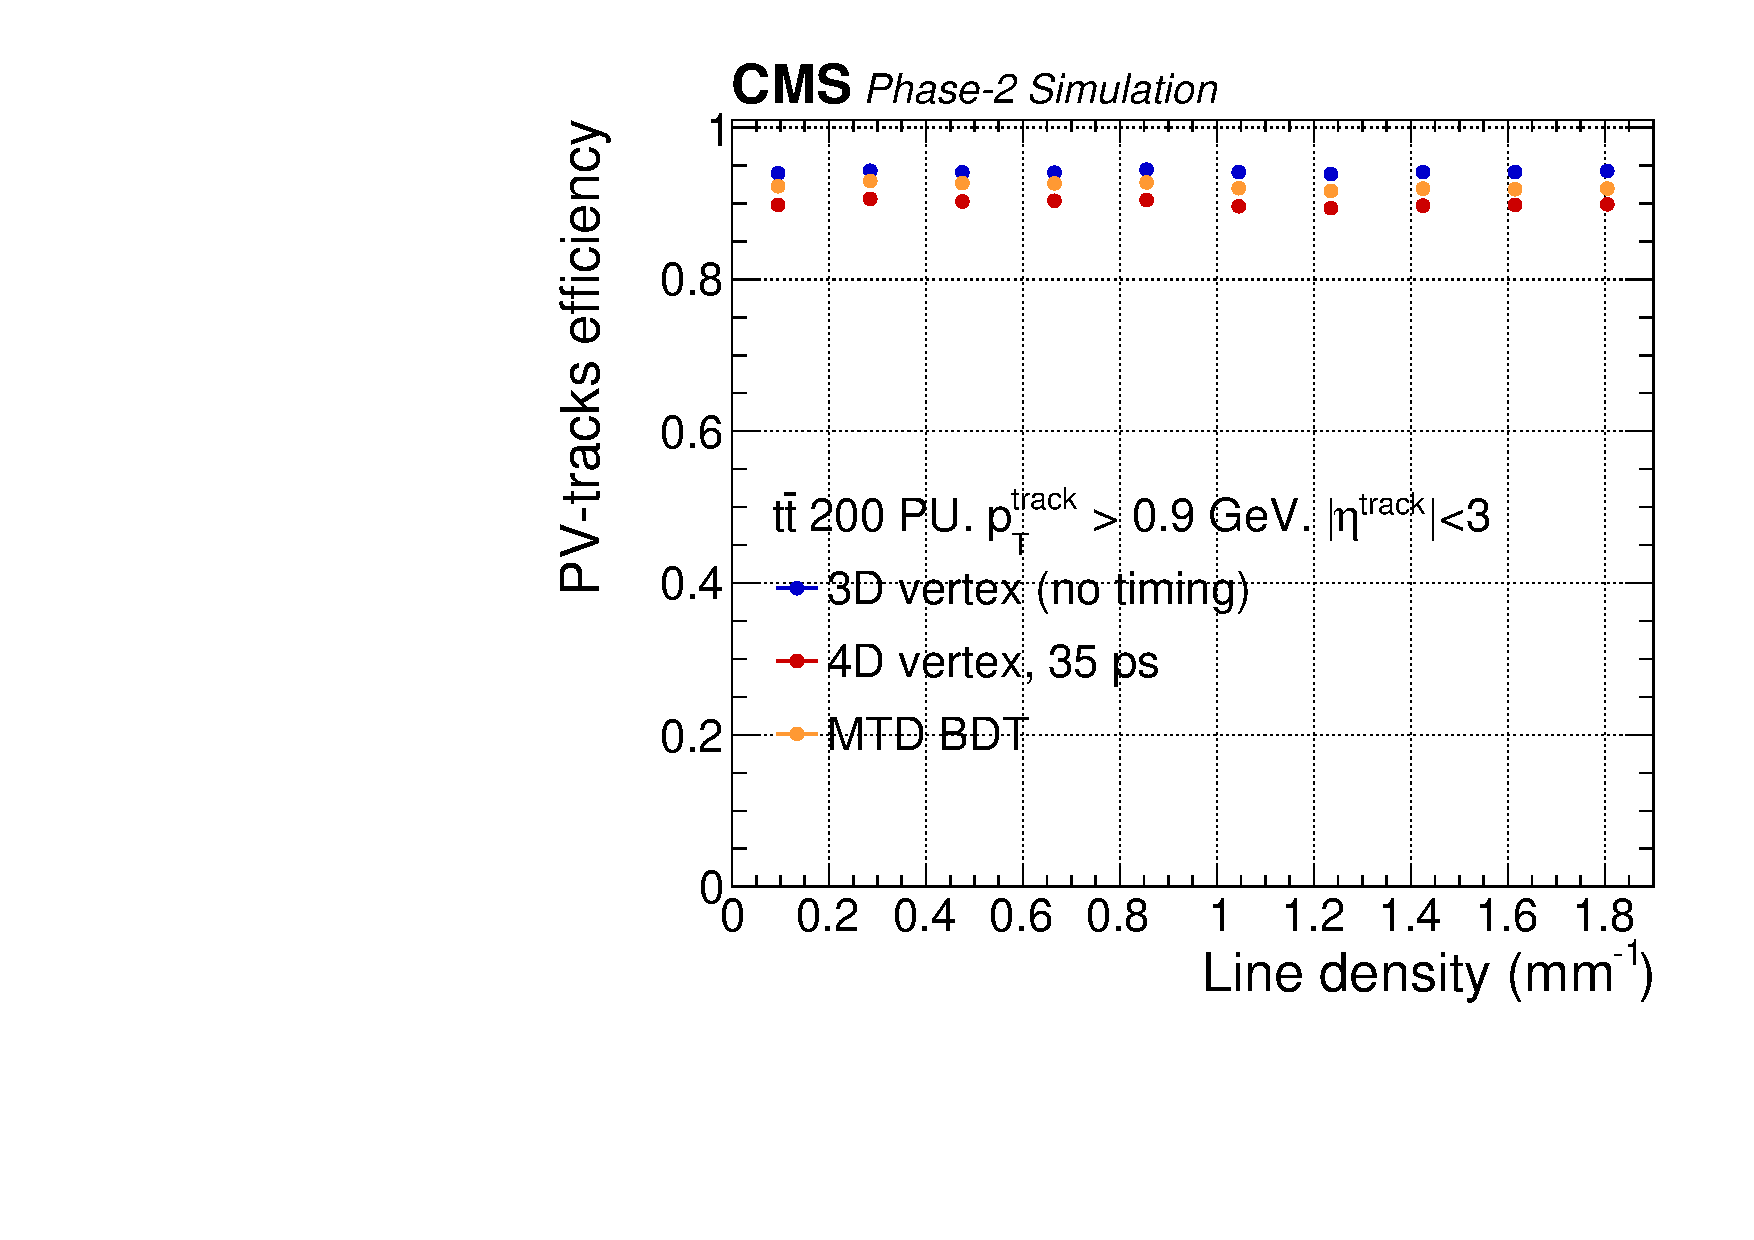
\includegraphics[width=0.48\textwidth]{fig/performance/purej/BDT_noTrackInfo/track_eff_vs_linden_ttbar.pdf}
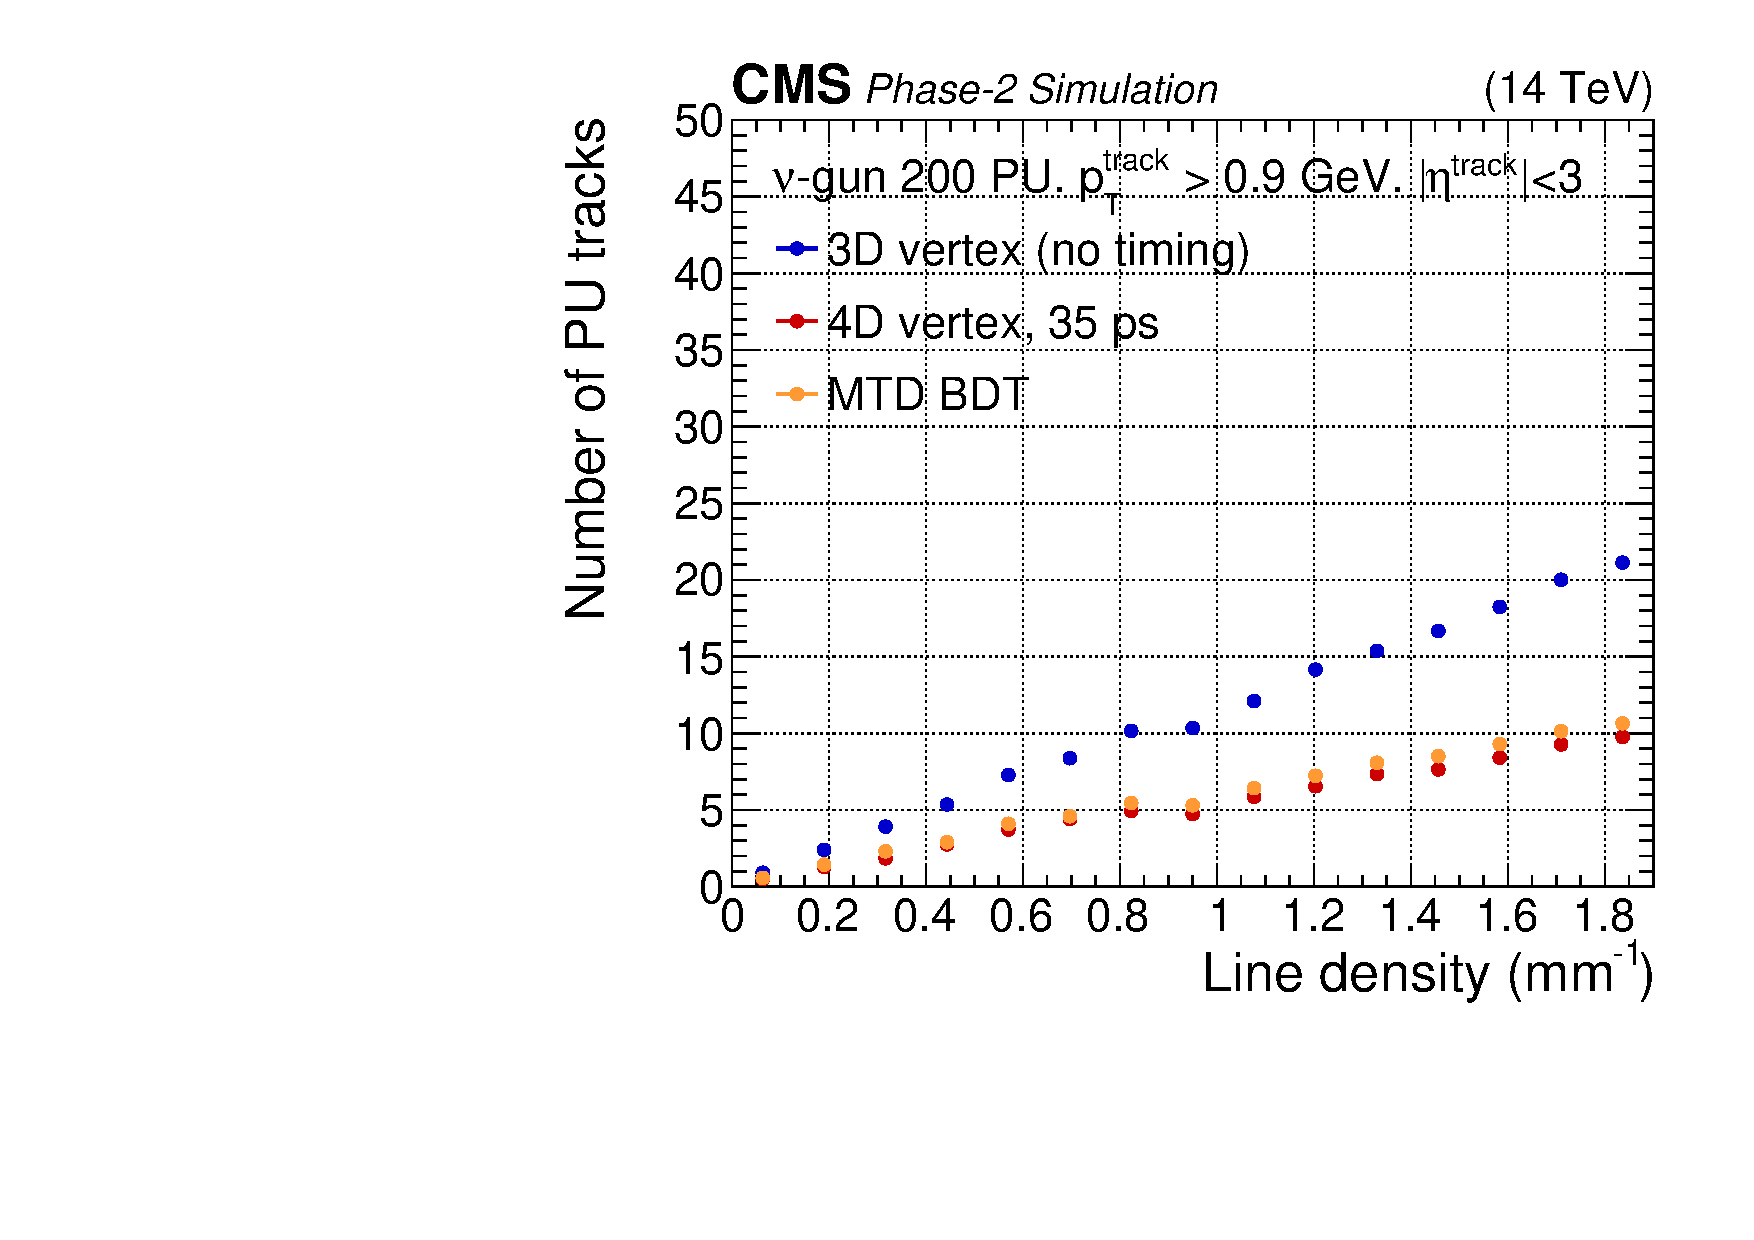
\includegraphics[width=0.48\textwidth]{fig/performance/purej/BDT_noTrackInfo/track_pu_vs_linden_nugun.pdf}
 \caption{Primary vertex association efficiency (left) and rejection (right) as a function of the line-density for primary vertex gen-matched tracks with different association criteria: blue $|\delta_{z}|<1$~mm,  red $|\delta_{z}|<1$~mm and $|\delta_{t}|<3\sigma_{t}$, orange $|\delta_{z}|<1$~mm and $BDT_{MTD}<WP_{95}$.  }
   \label{fig:purej_bdt}
\end{figure}

Further improvements to this approach can be clearly obtained using also the impact parameters in the longitudinal direction and in the transverse direction in the training of the multivariate classifier, which will be able to fully exploit the correlations between the track quality, track-MTD matching and 4D track-vertex impact parameters. 

It is useful also to compare the pile-up rejection capabilities with different time resolution using the fast-sim approach. Different time resolutions (30,40 and 50~ps) are compared in Fig.~\ref{fig:purej_tres_comp}, showing that the pile-up rejection capabilities are reduced of about 30\% going from a single track resolution of 30~ps to 50~ps.

\begin{figure}[!phtb]
\centering
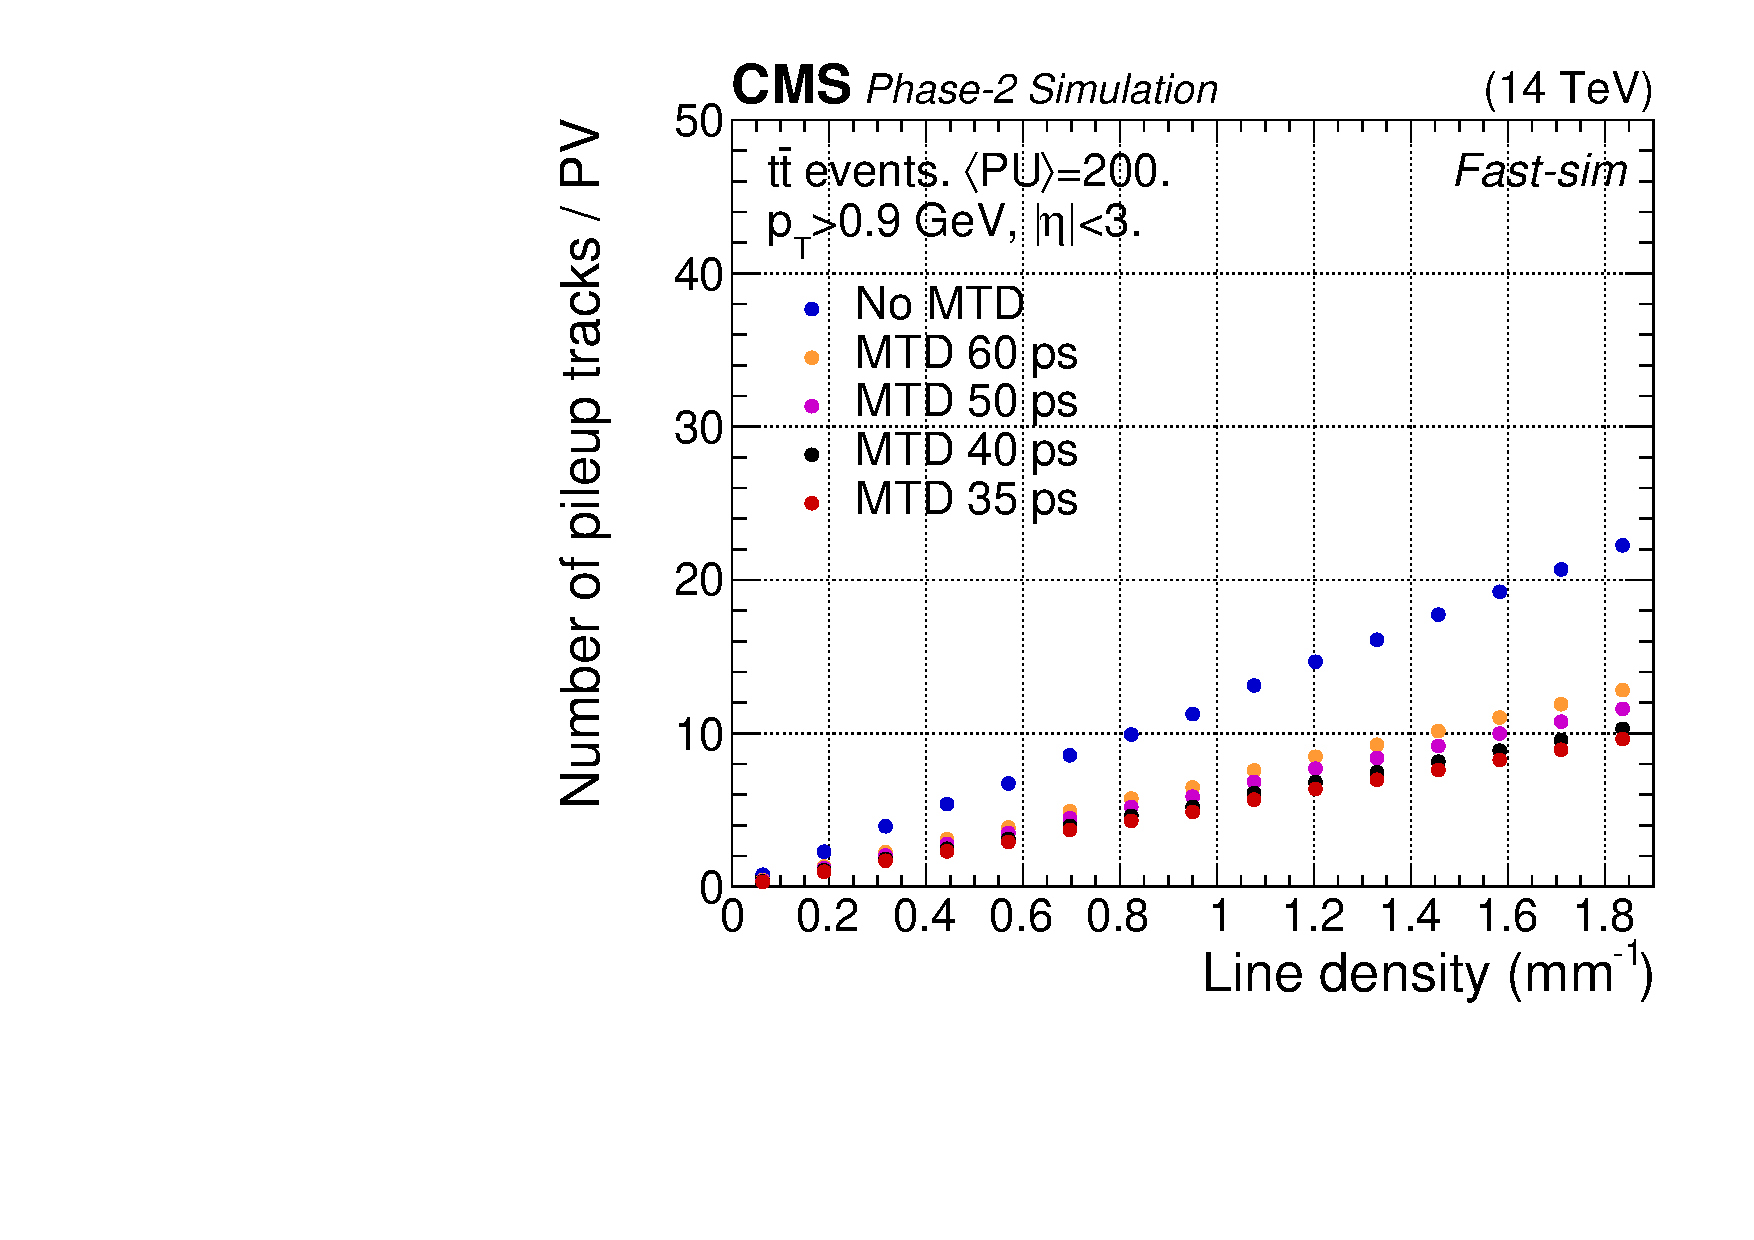
\includegraphics[width=0.48\textwidth]{fig/performance/purej/ForApproval/nputracks_fastsim_tres.pdf}
 \caption{Number of tracks from pileup incorrectly 
   associated with the hard primary vertex in \ttbar events from fast timing
   simulation as a function of the pileup density for different time resolutions.}
   \label{fig:purej_tres_comp}
\end{figure}
%%PM decide wether or not to discuss what can be achived with a Full4D BDT approach when compared 
